\documentclass{article}

\usepackage{fancyhdr}
\usepackage{extramarks}
\usepackage{amsmath}
\usepackage{amsthm}
\usepackage{amsfonts}
\usepackage{tikz}
\usepackage[plain]{algorithm}
\usepackage{algpseudocode}
\usepackage{physics}

\usetikzlibrary{automata,positioning}

%
% Basic Document Settings
%

\topmargin=-0.45in
\evensidemargin=0in
\oddsidemargin=0in
\textwidth=6.5in
\textheight=9.0in
\headsep=0.25in

\linespread{1.1}

\pagestyle{fancy}
\lhead{\hmwkAuthorName}
\chead{\hmwkClass\ (\hmwkClassInstructor\ \hmwkClassTime): \hmwkTitle}
\rhead{\firstxmark}
\lfoot{\lastxmark}
\cfoot{\thepage}

\renewcommand\headrulewidth{0.4pt}
\renewcommand\footrulewidth{0.4pt}

\setlength\parindent{0pt}

%
% Create Problem Sections
%

\newcommand{\enterProblemHeader}[1]{
    \nobreak\extramarks{}{Problem \arabic{#1} continued on next page\ldots}\nobreak{}
    \nobreak\extramarks{Problem \arabic{#1} (continued)}{Problem \arabic{#1} continued on next page\ldots}\nobreak{}
}

\newcommand{\exitProblemHeader}[1]{
    \nobreak\extramarks{Problem \arabic{#1} (continued)}{Problem \arabic{#1} continued on next page\ldots}\nobreak{}
    \stepcounter{#1}
    \nobreak\extramarks{Problem \arabic{#1}}{}\nobreak{}
}

\setcounter{secnumdepth}{0}
\newcounter{partCounter}
\newcounter{homeworkProblemCounter}
\setcounter{homeworkProblemCounter}{1}
\nobreak\extramarks{Problem \arabic{homeworkProblemCounter}}{}\nobreak{}

%
% Homework Problem Environment
%
% This environment takes an optional argument. When given, it will adjust the
% problem counter. This is useful for when the problems given for your
% assignment aren't sequential. See the last 3 problems of this template for an
% example.
%
\newenvironment{homeworkProblem}[1][-1]{
    \ifnum#1>0
        \setcounter{homeworkProblemCounter}{#1}
    \fi
    \section{Problem \arabic{homeworkProblemCounter}}
    \setcounter{partCounter}{1}
    \enterProblemHeader{homeworkProblemCounter}
}{
    \exitProblemHeader{homeworkProblemCounter}
}

%
% Homework Details
%   - Title
%   - Due date
%   - Class
%   - Section/Time
%   - Instructor
%   - Author
%

\newcommand{\hmwkTitle}{Assignment 2}
\newcommand{\hmwkDueDate}{February 05, 2024}
\newcommand{\hmwkClass}{COMP 4200}
\newcommand{\hmwkClassTime}{001}
\newcommand{\hmwkClassInstructor}{Professor Kwon}
\newcommand{\hmwkAuthorName}{\textbf{Matthew Rogers}}

%
% Title Page
%

\title{
    \vspace{2in}
    \textmd{\textbf{\hmwkClass:\ \hmwkTitle}}\\
    \normalsize\vspace{0.1in}\small{Due\ on\ \hmwkDueDate}\\
    \vspace{0.1in}\large{\textit{\hmwkClassInstructor\ \hmwkClassTime}}
    \vspace{3in}
}

\author{\hmwkAuthorName}
\date{}

\renewcommand{\part}[1]{\textbf{\large Part \Alph{partCounter}}\stepcounter{partCounter}\\}

%
% Various Helper Commands
%

% Useful for algorithms
\newcommand{\alg}[1]{\textsc{\bfseries \footnotesize #1}}

% For derivatives
\newcommand{\deriv}[1]{\frac{\mathrm{d}}{\mathrm{d}x} (#1)}

% For partial derivatives
\newcommand{\pderiv}[2]{\frac{\partial}{\partial #1} (#2)}

% Integral dx
\newcommand{\dx}{\mathrm{d}x}

% Alias for the Solution section header
\newcommand{\solution}{\textbf{\large Solution}}

% Probability commands: Expectation, Variance, Covariance, Bias
\newcommand{\E}{\mathrm{E}}
\newcommand{\Var}{\mathrm{Var}}
\newcommand{\Cov}{\mathrm{Cov}}
\newcommand{\Bias}{\mathrm{Bias}}

\begin{document}

\maketitle

\pagebreak

\begin{homeworkProblem}
    Draw the state diagram of DFAs recognizing the following languages.

    \begin{enumerate}
        \item A = $\{w \mid \abs{w} \text{ is a multiple of 3}\}$
        \item B = $\{11, 111\}$
        \item C = $\{w \mid w \text{ contains an even number of 0's and two 1's}\}$
        \item D = $\{w \mid w \text{ begins with 0 and every } w \text{ is preceded by 1}\}$
    \end{enumerate}

    \textbf{Solution}
    \\
    \\
    \textbf{Part One}

    \begin{figure}[h]
        \centering
        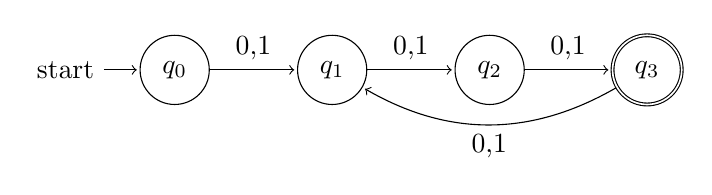
\begin{tikzpicture}[shorten >=1pt,node distance=2cm,on grid,auto]
            \node[state, initial] (q_0)   {$q_0$};
            \node[state] (q_1) [right=of q_0] {$q_1$};
            \node[state] (q_2) [right=of q_1] {$q_2$};
            \node[state, accepting,] (q_3) [right=of q_2] {$q_3$};
            \path[->]
                (q_0)
                    edge node {0,1} (q_1)
                (q_1)
                    edge node {0,1} (q_2)
                (q_2)
                    edge node {0,1} (q_3)
                (q_3)
                    edge [bend left] node {0,1} (q_1);
        \end{tikzpicture}
    \end{figure}

    \textbf{Part Two}

    \begin{figure}[h]
        \centering
        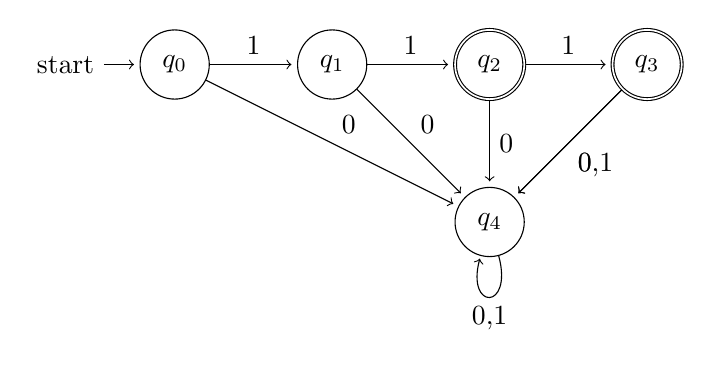
\begin{tikzpicture}[shorten >=2pt,node distance=2cm,on grid,auto]
            \node[state, initial] (q_0)   {$q_0$};
            \node[state] (q_1) [right=of q_0] {$q_1$};
            \node[state, accepting] (q_2) [right=of q_1] {$q_2$};
            \node[state, accepting] (q_3) [right=of q_2] {$q_3$};
            \node[state] (q_4) [below=of q_2] {$q_4$};
            \path[->]
                (q_0)
                    edge node {1} (q_1)
                    edge node {0} (q_4)
                (q_1)
                    edge node {1} (q_2)
                    edge node {0} (q_4)
                (q_2)
                    edge node {1} (q_3)
                    edge node {0} (q_4)
                (q_3)
                    edge node {0,1} (q_4)
                    edge node {0} (q_4)
                (q_4)
                    edge [loop below] node {0,1} (q_1);
        \end{tikzpicture}
    \end{figure}

    \textbf{Part Three}

    \begin{figure}[h]
        \centering
        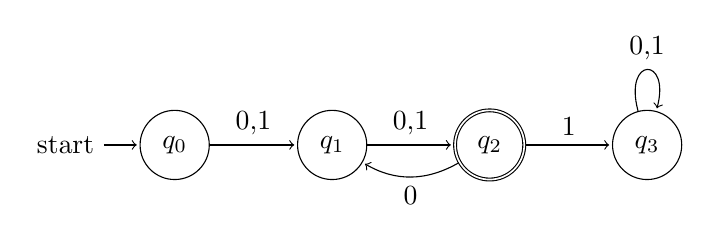
\begin{tikzpicture}[shorten >=1pt,node distance=2cm,on grid,auto]
            \node[state, initial] (q_0)   {$q_0$};
            \node[state] (q_1) [right=of q_0] {$q_1$};
            \node[state, accepting] (q_2) [right=of q_1] {$q_2$};
            \node[state] (q_3) [right=of q_2] {$q_3$};
            \path[->]
                (q_0)
                    edge node {0,1} (q_1)
                (q_1)
                    edge node {0,1} (q_2)
                (q_2)
                    edge node {1} (q_3)
                    edge [bend left] node {0} (q_1) 
                (q_3)
                    edge [loop above] node {0,1} (q_3);
        \end{tikzpicture}
    \end{figure}
    
    \textbf{Part Four}

    \begin{figure}[h]
        \centering
        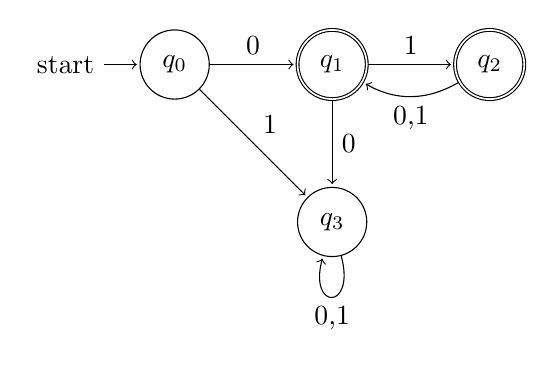
\begin{tikzpicture}[shorten >=1pt,node distance=2cm,on grid,auto]
            \node[state, initial] (q_0)   {$q_0$};
            \node[state, accepting] (q_1) [right=of q_0] {$q_1$};
            \node[state, accepting] (q_2) [right=of q_1] {$q_2$};
            \node[state] (q_3) [below=of q_1] {$q_3$};
            % \node[state] (q_4) [below=of q_2] {$q_4$};
            \path[->]
                (q_0)
                    edge node {0} (q_1)
                    edge node {1} (q_3)
                (q_1)
                    edge node {1} (q_2)
                    edge node {0} (q_3)
                (q_2)
                    edge [bend left] node {0,1} (q_1)
                (q_3)
                    edge [loop below] node {0,1} (q_3);
                % (q_4)
                %     edge [loop below] node {0,1} (q_1);
        \end{tikzpicture}
    \end{figure}

\end{homeworkProblem}

\pagebreak

\begin{homeworkProblem}
    Prove that regular languages are closed under set difference.

    \textbf{Solution}
    \\
    \\
    We will prove by construction, showing that $A-B$ is closed by creating it from other set operations.
    \\\newline
    We think of $A-B$ as \textit{everything that is in A that is also not in B}.
    $$A-B = A \cap \overline{B}$$
    Using the following properties of regular languages A and B,
    \begin{enumerate}
        \item $A \cap B$ is regular
        \item $\overline{A}$ is regular
    \end{enumerate}

    Given $A$, $B$ are regular languages,
    $$\overline{B} \text{ is regular}$$
    $$A \cap \overline{B} \text{ is regular}$$
    $$A-B \text{ is regular}$$
    \qed


\end{homeworkProblem}
\end{document}